\subsubsection{Control}

%% MIKKEL %%
% Hvordan og hvornår opdateres modellen?
% Hvordan dræbes brikker? Bliver de slettet eller skjult?
\textbf{Opdatering af modellen:} Brættet opdateres af metoden updateBoard i klassen \texttt{Control}. Når en brik er blevet flyttet, sætter \texttt{updateBoard} det brikkens nye felt optaget, og det tidligere felt frit.

Når en brik dræbes, køres metoden \texttt{removePiece} fra \texttt{DamModel}. \texttt{removePiece} sletter den dræbte brik fra \texttt{ArrayListen pieces}, fjerner brikken fra \texttt{Layoutet root}, og sætter brikkens tidligere felt til frit. Herefter skiftes fieldet \texttt{turnPlayer} værdi til den anden spiller. \texttt{turnPlayer} starter med at være \texttt{Player.Upper}, svarende til spilleren med de sorte brikker.\\

%% MIKKEL %%
% Hvordan styres et helt træk med en brik
\textbf{Legalt træk:} Når en brik slippes, køres metoden \texttt{isLegalMove} i klassen \texttt{Control}. \texttt{isLegalMove} afgør om trækket var legalt ved brug af metoderne i figur \ref{fig:tjekliste}:


\begin{figure}[H]
\centering
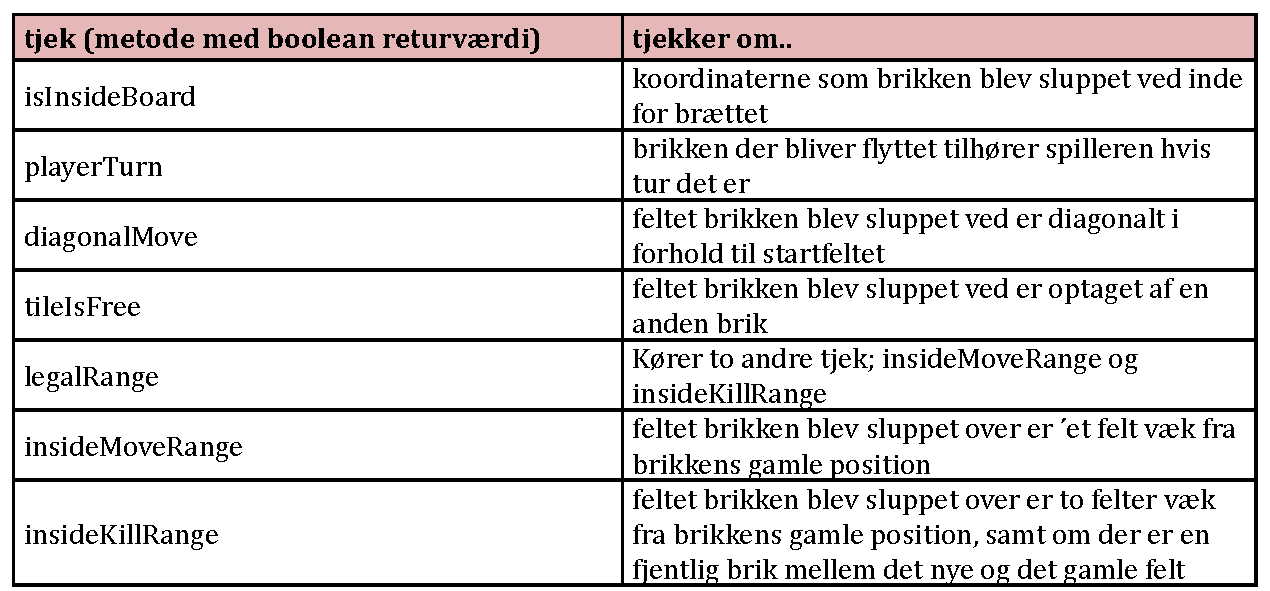
\includegraphics[width = 1.0  \textwidth]{Figurer/tjekliste.pdf}
\caption{Alle de forskellige tjek der bliver kørt i \texttt{isLegalMove}, og hvad de tjekker.}
\label{fig:tjekliste}
\end{figure}

De fleste at metoderne i figur \ref{fig:tjekliste} er accessors, der returnerer booleans. Metoden \texttt{insideKillRange} adskiller sig ved ikke blot at returnere en værdi, men også at være en mutator. Først tjekkes, om feltet mellem slutfeltet og startfeltet er optaget. Hvis dette er sandt, køres et \texttt{for-loop} over \texttt{ArrayListen pieces}, indtil der findes en brik med de feltets koordinater. Denne bliver nu gemt som \texttt{enemyPiece}. Derefter tjekkes, om strækningens længde er legal, og om \texttt{enemyPiece} tilhører fjendens hold. Dette tjek bliver gemt i en boolean \texttt{killPossible}. 

Hvis alle de tjeks i figur \ref{fig:tjekliste} er sande sættes boolean \texttt{moveIsLegal} til sand, så må brikken flyttes. Brættet opdateres.
